%!TEX root = ../thesis.tex

\ifpdf
    \graphicspath{{Chapter3/bs/Figs/Raster/}{Chapter3/bs/Figs/PDF/}{Chapter3/bs/Figs/}}
\else
    \graphicspath{{Chapter3/bs/Figs/Vector/}{Chapter3/bs/Figs/}}
\fi

\begin{figure}[htbp!]
\centering
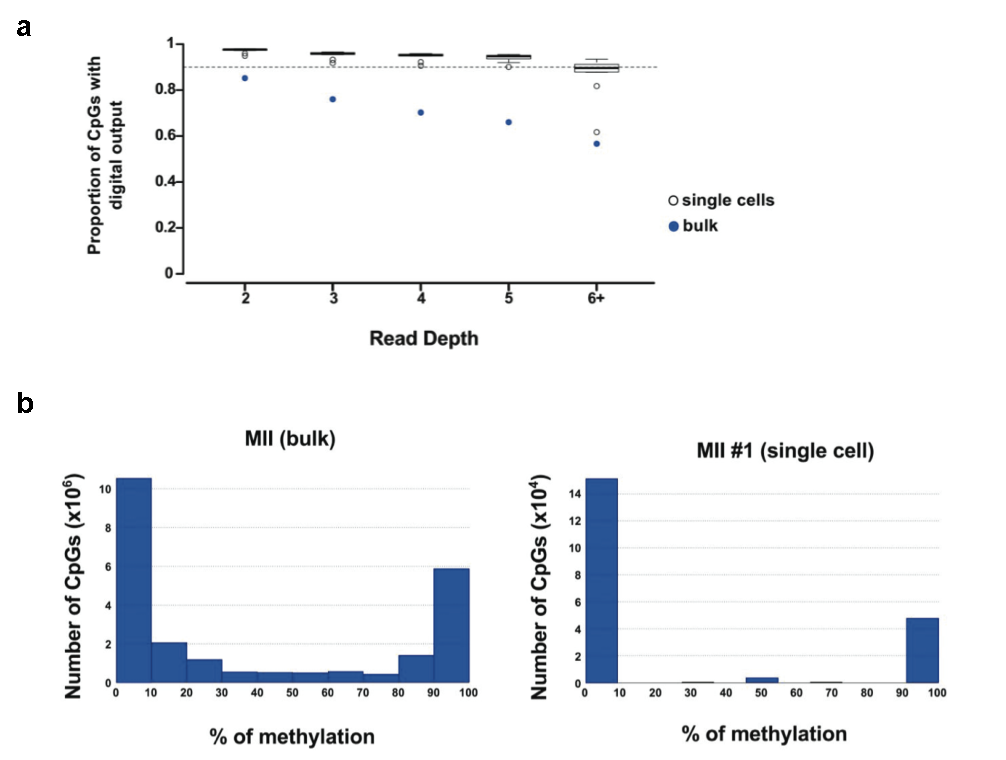
\includegraphics[width=1.0\textwidth]{binary}
\caption[scBS-seq generates a digital output of DNA methylation.]{scBS-seq generates a digital output of DNA methylation. (a) For each single MII BS-Seq library, and for the bulk MII sample, CpGs were grouped based on their read depth. The proportion of CpGs in each group with a methylation value of either 0\% or 100\% (digital output) was calculated for each sample. The boxplot represents the results from all 12 single MII libraries. The results from the bulk MII sample are superimposed as solid blue circles. As expected, the proportion of digital CpGs in the scBS-Seq libraries was very high ($>90\%$ for read depth 2-5 in all cells, dashed line). In contrast, the bulk sample had fewer digital CpGs (66\% at read depth 5) due to cell-to-cell variability within the population. (b) Histograms of the distribution of CpG methylation values for MII bulk and MII single cells for CpGs with at least 2 reads.}
\label{fig:bs_binary}
\end{figure}
